\documentclass[12pt,titlepage]{article}
\usepackage[margin=1.25in]{geometry}
\usepackage{graphicx,amsmath,minted}

%% Variables definition
\newcommand{\vSubject}{Data Structure and Algorithm Practicum}
\newcommand{\vSubtitle}{Double Linked List}
\newcommand{\vName}{Dicha Zelianivan Arkana}
\newcommand{\vNIM}{2241720002}
\newcommand{\vClass}{1i}
\newcommand{\vDepartment}{Information Technology}
\newcommand{\vStudyProgram}{D4 Informatics Engineering}

%% [START] Tikz related stuff
\usepackage{tikz}
\usetikzlibrary{svg.path,calc,shapes.geometric,shapes.misc}
\tikzstyle{terminator} = [rectangle, draw, text centered, rounded corners = 1em, minimum height=2em]
\tikzstyle{preparation} = [chamfered rectangle, chamfered rectangle sep=0.75em, draw, text centered, minimum height = 2em]
\tikzstyle{process} = [rectangle, draw, text centered, minimum height=2em]
\tikzstyle{decision} = [diamond, aspect=2, draw, text centered, minimum height=2em]
\tikzstyle{data}=[trapezium, draw, text centered, trapezium left angle=60, trapezium right angle=120, minimum height=2em]
\tikzstyle{connector} = [line width=0.25mm,->]
%% [END] Tikz related stuff

%% [START] Fancy header related stuff
\usepackage{fancyhdr}
\pagestyle{fancy}
\setlength{\headheight}{15pt} % compensate fancyhdr style
\fancyhead{}
\fancyfoot{}
\fancyfoot[L]{\thepage}
\fancyfoot[R]{\textit{\vSubject - \vSubtitle}}
\renewcommand{\footrulewidth}{0.4pt}% default is 0pt, overline for footer
%% [END] Fancy header related stuff

%% [START] Custom tabular command related stuff
\usepackage{tabularx}
\newcommand{\details}[2]{
    #1 & #2  \\
}
%% [END] Custom tabular command related stuff

%% [START] Figure related stuff
\newcommand{\image}[3][1]{
    \begin{figure}[h]
        \centering
        \includegraphics[#1]{#2}
        \caption{#3}
        \label{#3}
    \end{figure}
}
%% [END] Figure related stuff

\begin{document}
\begin{titlepage}
    \centering
    \vfill
    {\bfseries\LARGE
        \vSubject\\
        \vskip0.25cm
        \vSubtitle
    }
    \vfill
    
\includegraphics[width=6cm]{images/polinema-logo.png}
    \vfill
    {
        \textbf{Name}\\
        \vName\\
        \vskip0.5cm
        \textbf{NIM}\\
        \vNIM\\
        \vskip0.5cm
        \textbf{Class}\\
        \vClass\\
        \vskip0.5cm
        \textbf{Department}\\
        \vDepartment\\
        \vskip0.5cm
        \textbf{Study Program}\\
        \vStudyProgram
    }
\end{titlepage}

\section*{Lab Activity \#1}
\subsection*{Questions}
\begin{enumerate}
    \item {
        What's the difference between single linked list and double linked list?

        Single linked list only keep tracks of its next node while the double linked list
        keeps both the previous and the next node making it capable of traversing backwards.
    }
    \item {
        In \textbf{Node Class}, what is the usage of attribute next and prev?

        It's used to store the next and the previous pointer of the node in the linked list.
    }
    \item {
        In constructor of \textbf{DoubleLinkedList class}, what's the purpose of head and size attribute
        in this following code?

        \begin{minted}[autogobble,fontsize=\small]{java}
            public DoubleLinkedList() {
                head = null;
                size = 0;
            }
        \end{minted}

        It sets the initial value of the head, which is null since we haven't added any value yet.
        It also sets the initial value of the linked list size, which is zero because there are no items yet.
    }
    \item {
        In method \texttt{addFirst()}, why do we initialise the value of the Node object to be null at first?

        \begin{minted}[autogobble,fontsize=\small]{java}
            Node newNode = new Node(null, item, head);
        \end{minted}

        Because we're dealing with DoubleLinkedList, we also have the previous node. Since we're adding the first node,
        there is no previous node for a first node, which is why we set it to null.
    }
    \item {
        In method \texttt{addLast()}, what's the purpose of creating a node object by passing the \texttt{prev} parameter
        with \texttt{current} and \texttt{next} with \texttt{null}?

        \begin{minted}[autogobble,fontsize=\small]{java}
            Node newNode = new Node(current, item, null);
        \end{minted}

        The last element have its \texttt{next} value as null since it's the last element of the list.
        If the next node is not null then it won't be the last element of the list.
    }
\end{enumerate}

\section*{Lab Activities \#2}
\subsection*{Questions}
\begin{enumerate}
    \item {
        What's the meaning of these statements in \texttt{removeFirst()} method?
    }
    \item {
        How do we detect the position of the data that are in the last index in method \texttt{removeLast()}?
        
        We do that by checking if the \texttt{node.next.next} is null. If that conditions returns true,
        then we set the \texttt{node.next} to be null.
    }
    \item {
        Explain why this program code is not suitable if we include it in \texttt{remove} command!

        \begin{minted}[autogobble,fontsize=\small]{java}
            Node tmp = head.next;
            head.next = tmp.next;
            tmp.next.prev = head;
        \end{minted}

        It doesn't completely remove the current node since the current node will keep the reference of the head.
    }
    \item {
        Explain what's the function of this program code in method \texttt{remove}!

        \begin{minted}[autogobble,fontsize=\small]{java}
            current.prev.next = current.next;
            current.next.prev = current.prev;
        \end{minted}

        It's used to remove the current node by moving the \texttt{next} reference of the previous node into
        the \texttt{next} reference of the current node and then connecting the \texttt{prev} reference of the
        \texttt{next} node into the \texttt{prev} reference of the current node
    }
\end{enumerate}

\section*{Lab Activities \#3}
\subsection*{Questions}
\begin{enumerate}
    \item {
        What is the function of method \texttt{size()} in \textbf{DoubleLinkedList} class?

        It's to get the size of the linked list.
    }
    \item {
        How do we set the index in double linked list so that it starts from $1^{st}$ index instead of $0^{th}$ index?

        We need to set the first index as 1 in the constructor. This will make the consequent index to start from 1.
    }
    \item {
        Please explain the difference between method \texttt{add()} in double linked list and single linked list!

        In double linked list, we need to also handle the previous node. While in single linked list we can just attach the new node and only care about the \texttt{next} reference,
        we also need to care about the \texttt{prev} node in double linked list
    }
    \item {
        What's the logic difference of these 2 following codes?

        \begin{minted}[autogobble,fontsize=\small]{java}
            public boolean isEmpty() {
                if (size == 0) {
                    return true;
                } else {
                    return false;
                }
            }
        \end{minted}

        \begin{minted}[autogobble,fontsize=\small]{java}
            public boolean isEmpty() {
                return head == null;
            }
        \end{minted}

        The first one checks if the list is empty by checking its size while the second one checks if the head is null or not.
    }
\end{enumerate}

\section*{Assignment}
\begin{enumerate}
    \item {
        Create a program with double linked list implementation that allows user to choose a menu as
        following image! The searching uses sequential search approach and the program should be
        able to sort the data in descending order. You may choose any sorting approach you prefer
        (bubble sort, selection sort, insertion sort, or merge sort)

        \begin{figure}[h]
            \centering
            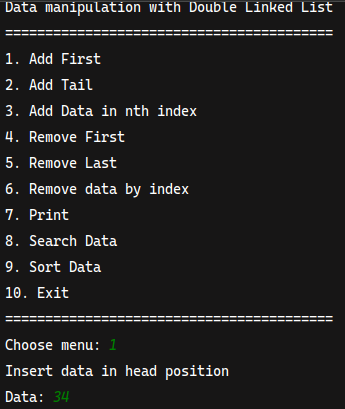
\includegraphics[width=0.25\textwidth]{./images/1-1.png}
            \caption{Inserting data from head}
        \end{figure}

        \begin{figure}[h]
            \centering
            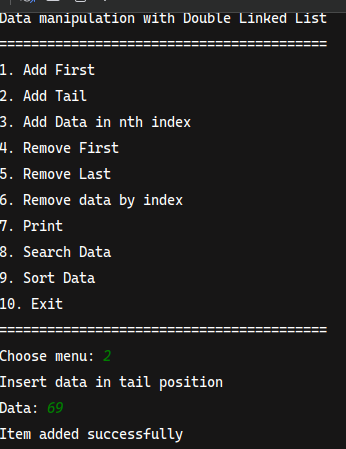
\includegraphics[width=0.25\textwidth]{./images/1-2.png}
            \caption{Inserting data from tail}
        \end{figure}

        \begin{figure}[h]
            \centering
            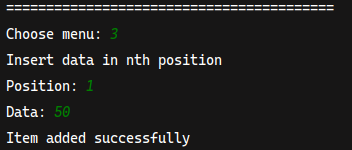
\includegraphics[width=0.25\textwidth]{./images/1-3.png}
            \caption{Inserting data in nth position}
        \end{figure}

        \pagebreak

        \begin{figure}[h]
            \centering
            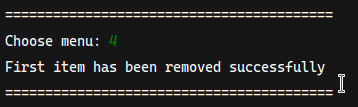
\includegraphics[width=0.25\textwidth]{./images/1-4.png}
            \caption{Remove the first data}
        \end{figure}

        \begin{figure}[h]
            \centering
            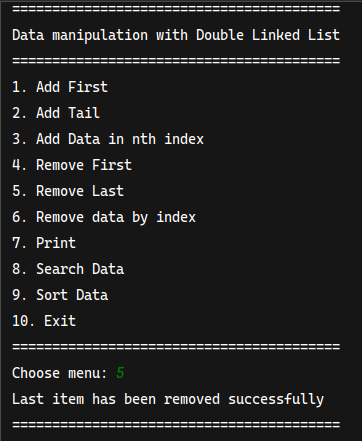
\includegraphics[width=0.25\textwidth]{./images/1-5.png}
            \caption{Remove the data in nth position}
        \end{figure}

        \begin{figure}[h]
            \centering
            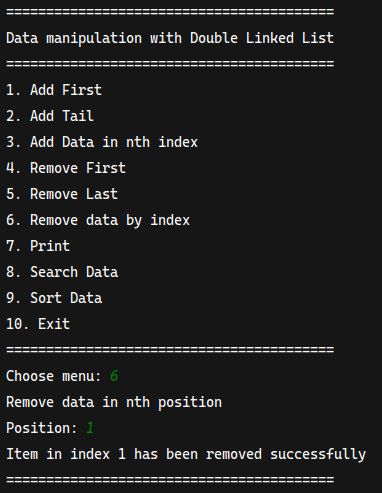
\includegraphics[width=0.25\textwidth]{./images/1-6.png}
            \caption{Remove the last data}
        \end{figure}

        \pagebreak

        \begin{figure}[h]
            \centering
            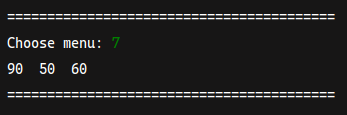
\includegraphics[width=0.25\textwidth]{./images/1-7.png}
            \caption{Remove the data in nth position}
        \end{figure}

        \begin{figure}[h]
            \centering
            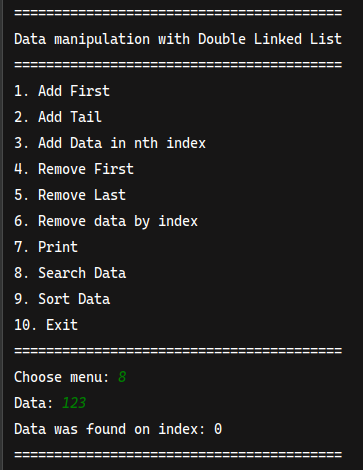
\includegraphics[width=0.25\textwidth]{./images/1-8.png}
            \caption{Remove the data in nth position}
        \end{figure}

        \pagebreak

        \large{\textbf{Node.java}}
        \begin{minted}[autogobble,fontsize=\small]{java}
            public class Node<T> {
                T data;
                Node<T> prev, next;

                public Node(Node<T> prev, T data, Node<T> next) {
                    this.prev = prev;
                    this.data = data;
                    this.next = next;
                }
            }
        \end{minted}

        \large{\textbf{DoubleLinkedListInteger.java}}

        \begin{minted}[autogobble,fontsize=\small]{java}
            public class DoubleLinkedListInteger {
                Node<Integer> head;
                int size;

                public DoubleLinkedListInteger() {
                    head = null;
                    size = 0;
                }

                boolean isEmpty() {
                    return size == 0;
                }

                void addFirst(Integer item) {
                    if (isEmpty()) {
                        head = new Node<>(null, item, null);
                    } else {
                        Node<Integer> newNode = new Node<>(null, item, head);
                        head.prev = newNode;
                        head = newNode;
                    }
                    size++;
                }

                void addLast(Integer item) {
                    if (isEmpty()) {
                        addFirst(item);
                        return;
                    }

                    Node<Integer> current = head;
                    while (current.next != null) {
                        current = current.next;
                    }
                    current.next = new Node<Integer>(current, item, null);
                    size++;
                }

                void addItem(Integer item, int index) throws Exception {
                    if (isEmpty()) {
                        addFirst(item);
                        return;
                    }

                    if (index < 0 || index > size) {
                        throw new Exception("Index out of bound");
                    }

                    Node<Integer> current = head;
                    int i = 0;
                    while (i < index) {
                        current = current.next;
                        i++;
                    }

                    if (current.next == null) {
                        Node<Integer> newNode = new Node<>(null, item, current);
                        current.prev = newNode;
                        head = newNode;
                    } else {
                        Node<Integer> newNode = new Node<>(current.prev, item, current);
                        newNode.prev = current.prev;
                        newNode.next = current;
                        current.prev.next = newNode;
                        current.prev = newNode;
                    }
                    size++;
                }

                int size() {
                    return size;
                }

                void clear() {
                    head = null;
                    size = 0;
                }

                void print() {
                    if (isEmpty()) {
                        System.out.println("Linked list is empty");
                        return;
                    }

                    Node<Integer> tmp = head;
                    while (tmp != null) {
                        System.out.print(tmp.data + "\t");
                        tmp = tmp.next;
                    }
                    System.out.println();
                }

                void removeFirst() throws Exception {
                    if (isEmpty()) {
                        throw new Exception("Linked list is still empty, cannot remove");
                    }

                    if (size == 1) {
                        removeLast();
                        return;
                    }

                    head = head.next;
                    head = null;
                    size--;
                }

                void removeLast() throws Exception {
                    if (isEmpty()) {
                        throw new Exception("Linked list is still empty, cannot remove");
                    }

                    if (head.next == null) {
                        head = null;
                    } else {
                        Node<Integer> current = head;
                        while (current.next.next != null) {
                            current = current.next;
                        }
                        current.next = null;
                    }
                    size--;
                }

                void remove(int index) throws Exception {
                    if (isEmpty() || index >= size) {
                        throw new Exception("Index value is out of bound");
                    }

                    if (index == 0) {
                        removeFirst();
                        return;
                    }

                    Node<Integer> current = head;
                    int i = 0;
                    while (i < index - 1) {
                        current = current.next;
                        i++;
                    }
                    current.next = current.next.next;
                    size--;
                }

                int getFirst() throws Exception {
                    if (isEmpty()) {
                        throw new Exception("Linked list is still empty");
                    }
                    return head.data;
                }

                int getLast() throws Exception {
                    if (isEmpty()) {
                        throw new Exception("Linked list is still empty");
                    }

                    Node<Integer> tmp = head;
                    while (tmp.next != null) {
                        tmp = tmp.next;
                    }
                    return tmp.data;
                }

                int get(int index) throws Exception {
                    if (isEmpty()) {
                        throw new Exception("Linked list is still empty");
                    }

                    Node<Integer> tmp = head;
                    for (int i = 0; i < index; i++) {
                        tmp = tmp.next;
                    }

                    return tmp.data;
                }

                int search(int data) {
                    if (isEmpty()) {
                        return -1;
                    }

                    Node<Integer> current = head;
                    int i = 0;
                    while (current.next != null) {
                        if (current.data == data) {
                            return i;
                        }
                        i++;
                        current = current.next;
                    }

                    return -1;
                }

                void bubbleSort() {
                    if (head == null || head.next == null) {
                        return; // No need to sort if the list is empty or has only one element
                    }

                    boolean swapped;
                    Node<Integer> current;
                    Node<Integer> last = null;

                    do {
                        swapped = false;
                        current = head;

                        while (current.next != last) {
                            if (current.data > current.next.data) {
                                swap(current, current.next);
                                swapped = true;
                            }
                            current = current.next;
                        }

                        last = current;
                    } while (swapped);
                }

                void swap(Node<Integer> left, Node<Integer> right) {
                    int temp = left.data;
                    left.data = right.data;
                    right.data = temp;
                }
            }
        \end{minted}

        \large{\textbf{DoubleLinkedListMain}}
        \begin{minted}[autogobble,fontsize=\small]{java}
            public class DoubleLinkedListMain {

            public static void main(String[] args) throws Exception {
                Scanner scanner = new Scanner(System.in);
                DoubleLinkedListInteger list = new DoubleLinkedListInteger();

                while (true) {
                    showMenu();
                    int chosenMenu = scanner.nextInt();
                    switch (chosenMenu) {
                        case 1: {
                            System.out.println("Insert data in head position");
                            System.out.print("Data: ");
                            int data = scanner.nextInt();
                            list.addFirst(data);
                            System.out.println("Item added successfully");
                            break;
                        }
                        case 2: {
                            System.out.println("Insert data in tail position");
                            System.out.print("Data: ");
                            int data = scanner.nextInt();
                            list.addLast(data);
                            System.out.println("Item added successfully");
                            break;
                        }
                        case 3: {
                            System.out.println("Insert data in nth position");
                            System.out.print("Position: ");
                            int position = scanner.nextInt();
                            System.out.print("Data: ");
                            int data = scanner.nextInt();
                            list.addItem(data, position);
                            System.out.println("Item added successfully");
                            break;
                        }
                        case 4: {
                            list.removeFirst();
                            System.out.println("First item has been removed successfully");
                            break;
                        }
                        case 5: {
                            list.removeLast();
                            System.out.println("Last item has been removed successfully");
                            break;
                        }
                        case 6: {
                            System.out.println("Remove data in nth position");
                            System.out.print("Position: ");
                            int position = scanner.nextInt();
                            list.remove(position);
                            System.out.printf("Item in index %s has been removed successfully\n", position);
                            break;
                        }
                        case 7: {
                            list.print();
                            break;
                        }
                        case 8: {
                            System.out.print("Data: ");
                            int data = scanner.nextInt();
                            int index = list.search(data);
                            if (index == -1) {
                                System.out.println("No data was found on the list");
                                break;
                            }
                            System.out.printf("Data was found on index: %s\n", index);
                            break;
                        }
                        case 9: {
                            list.bubbleSort();
                            break;
                        }
                        case 10: {
                            System.out.println("Exiting...");
                            break;
                        }
                        default: {
                            System.out.println("Invalid input");
                            return;
                        }
                    }
                }

            }

            static void showMenu() {
                System.out.println("=========================================");
                System.out.println("Data manipulation with Double Linked List");
                System.out.println("=========================================");
                System.out.println("1. Add First");
                System.out.println("2. Add Tail");
                System.out.println("3. Add Data in nth index");
                System.out.println("4. Remove First");
                System.out.println("5. Remove Last");
                System.out.println("6. Remove data by index");
                System.out.println("7. Print");
                System.out.println("8. Search Data");
                System.out.println("9. Sort Data");
                System.out.println("10. Exit");
                System.out.println("=========================================");
                System.out.print("Choose menu: ");
            }
        }
        \end{minted}

    }

    \pagebreak

    \item {
        We are required to create a program which implement Stack using double linked list. The
        features are described in following illustrations

        \begin{figure}[h]
            \centering
            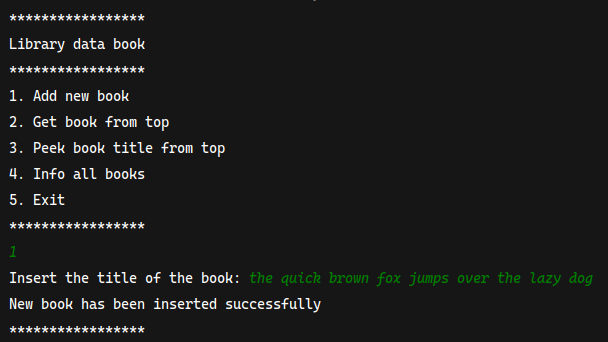
\includegraphics[width=0.5\textwidth]{./images/2-1.png}
            \caption{Add item}
        \end{figure}

        \begin{figure}[h]
            \centering
            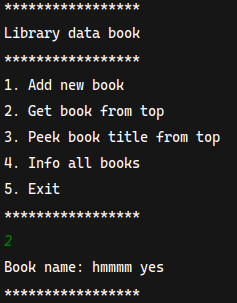
\includegraphics[width=0.25\textwidth]{./images/2-2.png}
            \caption{Get book from top of stack}
        \end{figure}

        \begin{figure}[h]
            \centering
            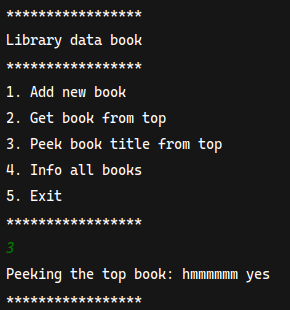
\includegraphics[width=0.25\textwidth]{./images/2-3.png}
            \caption{Peek book title from top}
        \end{figure}

        \pagebreak

        \begin{figure}[h]
            \centering
            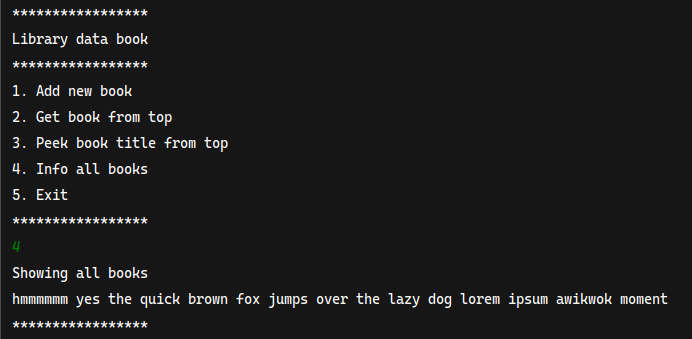
\includegraphics[width=0.5\textwidth]{./images/2-4.png}
            \caption{Info all books}
        \end{figure}

        \large{\textbf{StudentList.java}}
        \begin{minted}[autogobble,fontsize=\small]{java}
            public class StudentList {
                private final DoubleLinkedList<Student> list;

                public StudentList() {
                    list = new DoubleLinkedList<>();
                }

                // add data from head
                public void addFirst(Student data) {
                    list.addFirst(data);
                }

                // add data from tail
                public void addLast(Student data) {
                    list.addLast(data);
                }

                // add data in specific index from head
                public void addFrom(Student data, int index) throws Exception {
                    list.addItem(data, index);
                }

                // remove data from head
                public void removeFirst() throws Exception {
                    list.removeFirst();
                }

                // remove data from tail
                public void removeLast() throws Exception {
                    list.removeLast();
                }

                // remove data in specific index
                public void remove(int index) throws Exception {
                    list.remove(index);
                }

                // print
                public void print() {
                    Node<Student> current = list.head;
                    while (current != null) {
                        System.out.println("| " + current.data.nim + " | " + current.data.name + " | " + current.data.gpa + " |");
                        current = current.next;
                    }
                    System.out.println();
                }

                // search by nim
                public int search(String nim) {
                    if (list.isEmpty()) {
                        return -1;
                    }

                    Node<Student> current = list.head;
                    int i = 0;
                    while (current != null) {
                        if (current.data.nim.equals(nim)) {
                            return i;
                        }
                        current = current.next;
                        i++;
                    }
                    return -1;
                }

                // sort by gpa - desc
                public void sortByGpa() {
                    if (list.head == null || list.head.next == null) {
                        return; // No need to sort if the list is empty or has only one element
                    }

                    boolean swapped;
                    Node<Student> current;
                    Node<Student> last = null;

                    do {
                        swapped = false;
                        current = list.head;

                        while (current.next != last) {
                            if (current.data.gpa > current.next.data.gpa) {
                                swap(current, current.next);
                                swapped = true;
                            }
                            current = current.next;
                        }

                        last = current;
                    } while (swapped);
                }

                static void swap(Node<Student> left, Node<Student> right) {
                    Student tmp = left.data;
                    left.data = right.data;
                    right.data = tmp;
                }
            }
        \end{minted}

        \large{\textbf{StudentMain.java}}
        \begin{minted}[autogobble,fontsize=\small]{java}
            public class StudentMain {
                public static void main(String[] args) throws Exception {
                    Scanner scanner = new Scanner(System.in);
                    StudentList studentList = new StudentList();

                    while (true) {
                        showMenu();
                        int chosenMenu = scanner.nextInt();
                        switch (chosenMenu) {
                            case 1: {
                                System.out.println("Add data from head");
                                System.out.print("NIM: ");
                                scanner.nextLine();
                                String nim = scanner.nextLine();
                                System.out.print("Name: ");
                                String name = scanner.nextLine();
                                System.out.print("GPA: ");
                                double gpa = scanner.nextDouble();
                                Student student = new Student(nim, name, gpa);
                                studentList.addFirst(student);
                                break;
                            }
                            case 2: {
                                System.out.println("Add data from tail");
                                System.out.print("NIM: ");
                                scanner.nextLine();
                                String nim = scanner.nextLine();
                                System.out.print("Name: ");
                                String name = scanner.nextLine();
                                System.out.print("GPA: ");
                                double gpa = scanner.nextDouble();
                                Student student = new Student(nim, name, gpa);
                                studentList.addLast(student);
                                break;
                            }
                            case 3: {
                                System.out.println("Add data to specific index");
                                System.out.print("Index: ");
                                int index = scanner.nextInt();
                                scanner.nextLine();
                                System.out.print("NIM: ");
                                String nim = scanner.nextLine();
                                System.out.print("Name: ");
                                String name = scanner.nextLine();
                                System.out.print("GPA: ");
                                double gpa = scanner.nextDouble();
                                Student student = new Student(nim, name, gpa);
                                studentList.addFrom(student, index);
                                break;
                            }
                            case 4: {
                                System.out.println("Remove data from head");
                                studentList.removeFirst();
                                break;
                            }
                            case 5: {
                                System.out.println("Remove data from tail");
                                studentList.removeLast();
                                break;
                            }
                            case 6: {
                                System.out.println("Remove data in specific index");
                                System.out.print("Index: ");
                                int index = scanner.nextInt();
                                studentList.remove(index);
                                break;
                            }
                            case 7: {
                                System.out.println("Print");
                                studentList.print();
                                break;
                            }
                            case 8: {
                                System.out.println("Search by NIM");
                                System.out.print("NIM: ");
                                scanner.nextLine();
                                String nim = scanner.nextLine();
                                System.out.println("Index: " + studentList.search(nim));
                                break;
                            }
                            case 9: {
                                System.out.println("Sort by GPA");
                                studentList.sortByGpa();
                                break;
                            }
                            case 10: {
                                System.out.println("Exit");
                                return;
                            }
                        }
                    }
                }

                public static void showMenu() {
                    System.out.println("==============================");
                    System.out.println("Student Data Management System");
                    System.out.println("==============================");
                    System.out.println("1. Add data from head");
                    System.out.println("2. Add data from tail");
                    System.out.println("3. Add data to specific index");
                    System.out.println("4. Remove data from head");
                    System.out.println("5. Remove data from tail");
                    System.out.println("6. Remove data from specific index");
                    System.out.println("7. Print");
                    System.out.println("8. Search by NIM");
                    System.out.println("9. Sort by GPA");
                    System.out.println("10. Exit");
                    System.out.println("==============================");
                }
            }
        \end{minted}
    }
    \pagebreak
    \item {
        Create a program that helps vaccination process by having a queue algorithm alongside with
        double linked list as follows \textbf{(the amount left of queue length in menu print(3) and recent
        vaccinated person in menu Remove data (2) should be displayed)}!

        \begin{figure}[h]
            \centering
            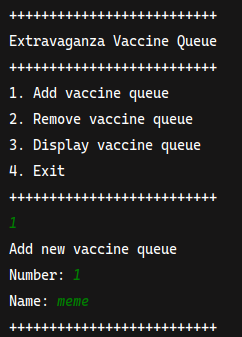
\includegraphics[width=0.25\textwidth]{./images/3-1.png}
            \caption{Add to queue}
        \end{figure}

        \begin{figure}[h]
            \centering
            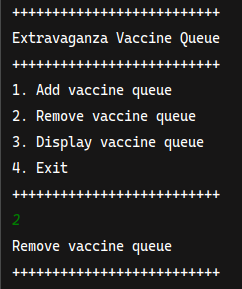
\includegraphics[width=0.25\textwidth]{./images/3-2.png}
            \caption{Remove from queue}
        \end{figure}

        \pagebreak

        \begin{figure}[h]
            \centering
            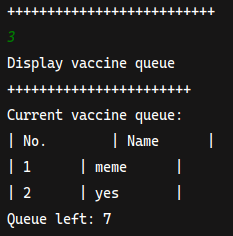
\includegraphics[width=0.25\textwidth]{./images/3-3.png}
            \caption{Display vaccine queue}
        \end{figure}

        \large{\textbf{Queue.java}}
        \begin{minted}[autogobble,fontsize=\small]{java}
            public class Queue {
                private final DoubleLinkedList<Patient> list;
                private int maxCapacity;
                private int currentCapacity;

                public Queue(int maxQueue) {
                    this.maxCapacity = maxQueue;
                    this.currentCapacity = 0;
                    this.list = new DoubleLinkedList<>();
                }

                public void add(Patient data) {
                    if (currentCapacity >= maxCapacity) {
                        System.out.println("List is already maxed out");
                        return;
                    }

                    list.addLast(data);
                    maxCapacity--;
                }

                public void remove() throws Exception {
                    if (currentCapacity == 0) {

                    }
                    list.removeFirst();
                    maxCapacity++;
                }

                public void display() {
                    System.out.println("+++++++++++++++++++++++");
                    System.out.println("Current vaccine queue: ");
                    System.out.println("| No.\t\t | Name\t\t |");

                    Node<Patient> tmp = list.head;
                    while (tmp.next != null) {
                        System.out.printf("| %d\t\t | %s\t\t |\n", tmp.data.number, tmp.data.name);
                        tmp = tmp.next;
                    }

                    System.out.printf("Queue left: %d\n", maxCapacity);
                    System.out.println("+++++++++++++++++++++++");
                }
            }
        \end{minted}

        \large{\textbf{QueueMain.java}}
        \begin{minted}[autogobble,fontsize=\small]{java}
            public class QueueMain {
                public static void main(String[] args) throws Exception {
                    Scanner scanner = new Scanner(System.in);
                    Queue patientQueue = new Queue(10);

                    while (true) {
                        showMenu();
                        int chosenMenu = scanner.nextInt();
                        switch (chosenMenu) {
                            case 1: {
                                System.out.println("Add new vaccine queue");
                                System.out.print("Number: ");
                                int number = scanner.nextInt();
                                System.out.print("Name: ");
                                scanner.nextLine();
                                String name = scanner.nextLine();
                                patientQueue.add(new Patient(number, name));
                                break;
                            }
                            case 2: {
                                System.out.println("Remove vaccine queue");
                                patientQueue.remove();
                                break;
                            }
                            case 3: {
                                System.out.println("Display vaccine queue");
                                patientQueue.display();
                                break;
                            }
                            case 4: {
                                System.out.println("Exit");
                                return;
                            }
                        }
                    }
                }

                static void showMenu() {
                    System.out.println("++++++++++++++++++++++++++");
                    System.out.println("Extravaganza Vaccine Queue");
                    System.out.println("++++++++++++++++++++++++++");
                    System.out.println("1. Add vaccine queue");
                    System.out.println("2. Remove vaccine queue");
                    System.out.println("3. Display vaccine queue");
                    System.out.println("4. Exit");
                    System.out.println("++++++++++++++++++++++++++");
                }
            }
        \end{minted}

    }
    \pagebreak
    \item {
        Create a program implementation that list students score. Each student’s data consist of their
        nim, name, and gpa. The program should implement double linked list and should be able to
        search based on NIM and sort the GPA in descending order. Students class must be
        implemented in this program!

        \begin{figure}[h]
            \centering
            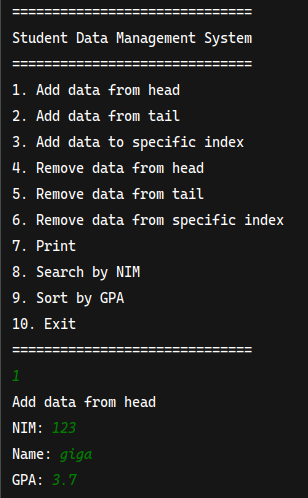
\includegraphics[width=0.25\textwidth]{./images/4-1.png}
            \caption{Add data from head}
        \end{figure}

        \begin{figure}[h]
            \centering
            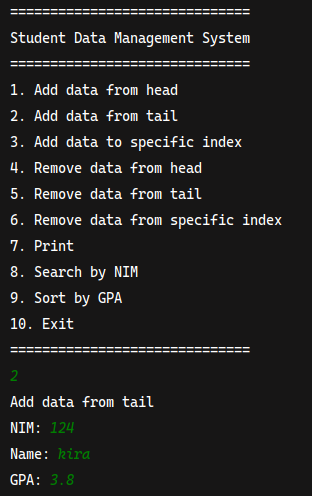
\includegraphics[width=0.25\textwidth]{./images/4-2.png}
            \caption{Add data from tail}
        \end{figure}

        \begin{figure}[h]
            \centering
            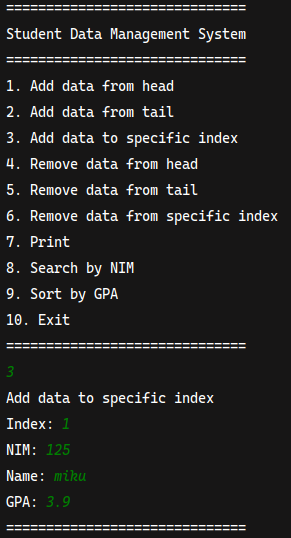
\includegraphics[width=0.25\textwidth]{./images/4-3.png}
            \caption{Add data to specific index}
        \end{figure}

        \pagebreak

        \begin{figure}[h]
            \centering
            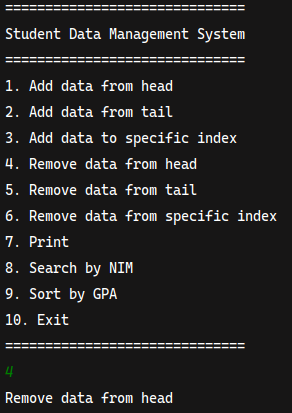
\includegraphics[width=0.25\textwidth]{./images/4-4.png}
            \caption{Remove data from head}
        \end{figure}

        \begin{figure}[h]
            \centering
            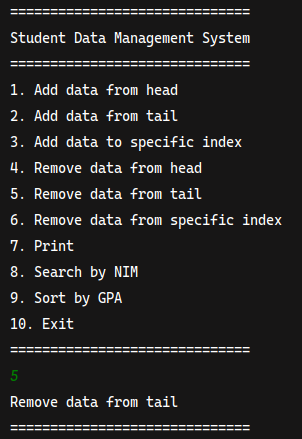
\includegraphics[width=0.25\textwidth]{./images/4-5.png}
            \caption{Remove data from tail}
        \end{figure}

        \pagebreak

        \begin{figure}[h]
            \centering
            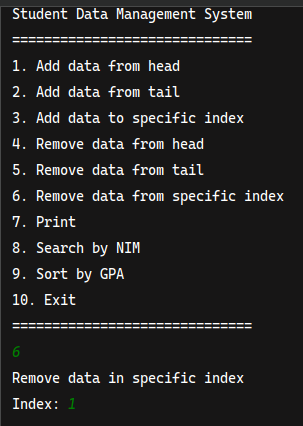
\includegraphics[width=0.25\textwidth]{./images/4-6.png}
            \caption{Remove data from specific index}
        \end{figure}

        \begin{figure}[h]
            \centering
            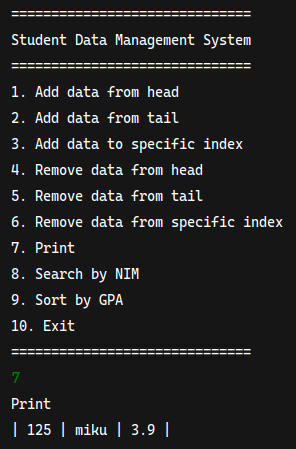
\includegraphics[width=0.25\textwidth]{./images/4-7.png}
            \caption{Display data}
        \end{figure}

        \pagebreak

        \begin{figure}[h]
            \centering
            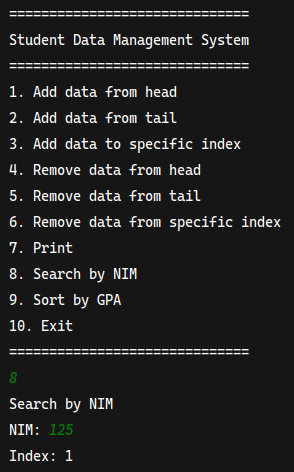
\includegraphics[width=0.25\textwidth]{./images/4-8.png}
            \caption{Search data}
        \end{figure}

        \pagebreak

        \begin{figure}[h]
            \centering
            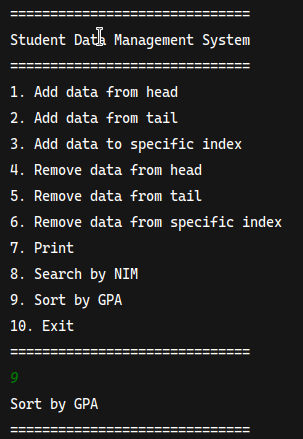
\includegraphics[width=0.25\textwidth]{./images/4-9-1.png}
            \caption{Sort data}
        \end{figure}

        \begin{figure}[h]
            \centering
            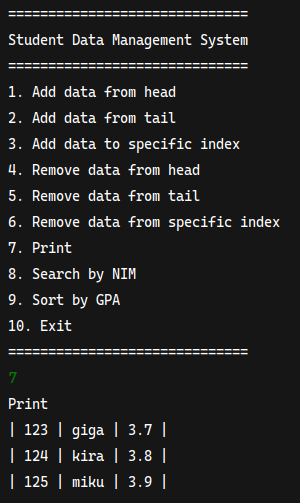
\includegraphics[width=0.25\textwidth]{./images/4-9-2.png}
            \caption{Sort data}
        \end{figure}

        \pagebreak

        \large{\textbf{Student.java}}
        \begin{minted}[autogobble,fontsize=\small]{java}
            public class Student {
                public String nim;
                public String name;
                public double gpa;

                public Student(String nim, String name, double gpa) {
                    this.nim = nim;
                    this.name = name;
                    this.gpa = gpa;
                }
            }
        \end{minted}

        \large{\textbf{StudentList.java}}
        \begin{minted}[autogobble,fontsize=\small]{java}
            public class StudentList {
                private final DoubleLinkedList<Student> list;

                public StudentList() {
                    list = new DoubleLinkedList<>();
                }

                // add data from head
                public void addFirst(Student data) {
                    list.addFirst(data);
                }

                // add data from tail
                public void addLast(Student data) {
                    list.addLast(data);
                }

                // add data in specific index from head
                public void addFrom(Student data, int index) throws Exception {
                    list.addItem(data, index);
                }

                // remove data from head
                public void removeFirst() throws Exception {
                    list.removeFirst();
                }

                // remove data from tail
                public void removeLast() throws Exception {
                    list.removeLast();
                }

                // remove data in specific index
                public void remove(int index) throws Exception {
                    list.remove(index);
                }

                // print
                public void print() {
                    Node<Student> current = list.head;
                    while (current != null) {
                        System.out.println("| " + current.data.nim + " | " + current.data.name + " | " + current.data.gpa + " |");
                        current = current.next;
                    }
                    System.out.println();
                }

                // search by nim
                public int search(String nim) {
                    if (list.isEmpty()) {
                        return -1;
                    }

                    Node<Student> current = list.head;
                    int i = 0;
                    while (current != null) {
                        if (current.data.nim.equals(nim)) {
                            return i;
                        }
                        current = current.next;
                        i++;
                    }
                    return -1;
                }

                // sort by gpa - desc
                public void sortByGpa() {
                    if (list.head == null || list.head.next == null) {
                        return; // No need to sort if the list is empty or has only one element
                    }

                    boolean swapped;
                    Node<Student> current;
                    Node<Student> last = null;

                    do {
                        swapped = false;
                        current = list.head;

                        while (current.next != last) {
                            if (current.data.gpa > current.next.data.gpa) {
                                swap(current, current.next);
                                swapped = true;
                            }
                            current = current.next;
                        }

                        last = current;
                    } while (swapped);
                }

                static void swap(Node<Student> left, Node<Student> right) {
                    Student tmp = left.data;
                    left.data = right.data;
                    right.data = tmp;
                }
            }
        \end{minted}

        \large{\textbf{StudentMain.java}}
        \begin{minted}[autogobble,fontsize=\small]{java}
            public class StudentMain {
                public static void main(String[] args) throws Exception {
                    Scanner scanner = new Scanner(System.in);
                    StudentList studentList = new StudentList();

                    while (true) {
                        showMenu();
                        int chosenMenu = scanner.nextInt();
                        switch (chosenMenu) {
                            case 1: {
                                System.out.println("Add data from head");
                                System.out.print("NIM: ");
                                scanner.nextLine();
                                String nim = scanner.nextLine();
                                System.out.print("Name: ");
                                String name = scanner.nextLine();
                                System.out.print("GPA: ");
                                double gpa = scanner.nextDouble();
                                Student student = new Student(nim, name, gpa);
                                studentList.addFirst(student);
                                break;
                            }
                            case 2: {
                                System.out.println("Add data from tail");
                                System.out.print("NIM: ");
                                scanner.nextLine();
                                String nim = scanner.nextLine();
                                System.out.print("Name: ");
                                String name = scanner.nextLine();
                                System.out.print("GPA: ");
                                double gpa = scanner.nextDouble();
                                Student student = new Student(nim, name, gpa);
                                studentList.addLast(student);
                                break;
                            }
                            case 3: {
                                System.out.println("Add data to specific index");
                                System.out.print("Index: ");
                                int index = scanner.nextInt();
                                scanner.nextLine();
                                System.out.print("NIM: ");
                                String nim = scanner.nextLine();
                                System.out.print("Name: ");
                                String name = scanner.nextLine();
                                System.out.print("GPA: ");
                                double gpa = scanner.nextDouble();
                                Student student = new Student(nim, name, gpa);
                                studentList.addFrom(student, index);
                                break;
                            }
                            case 4: {
                                System.out.println("Remove data from head");
                                studentList.removeFirst();
                                break;
                            }
                            case 5: {
                                System.out.println("Remove data from tail");
                                studentList.removeLast();
                                break;
                            }
                            case 6: {
                                System.out.println("Remove data in specific index");
                                System.out.print("Index: ");
                                int index = scanner.nextInt();
                                studentList.remove(index);
                                break;
                            }
                            case 7: {
                                System.out.println("Print");
                                studentList.print();
                                break;
                            }
                            case 8: {
                                System.out.println("Search by NIM");
                                System.out.print("NIM: ");
                                scanner.nextLine();
                                String nim = scanner.nextLine();
                                System.out.println("Index: " + studentList.search(nim));
                                break;
                            }
                            case 9: {
                                System.out.println("Sort by GPA");
                                studentList.sortByGpa();
                                break;
                            }
                            case 10: {
                                System.out.println("Exit");
                                return;
                            }
                        }
                    }
                }

                public static void showMenu() {
                    System.out.println("==============================");
                    System.out.println("Student Data Management System");
                    System.out.println("==============================");
                    System.out.println("1. Add data from head");
                    System.out.println("2. Add data from tail");
                    System.out.println("3. Add data to specific index");
                    System.out.println("4. Remove data from head");
                    System.out.println("5. Remove data from tail");
                    System.out.println("6. Remove data from specific index");
                    System.out.println("7. Print");
                    System.out.println("8. Search by NIM");
                    System.out.println("9. Sort by GPA");
                    System.out.println("10. Exit");
                    System.out.println("==============================");
                }
            }
        \end{minted}
    }
\end{enumerate}

\end{document}

